\section{Das iOS Betriebsystem}
	Die aus Cupertino in Kalifornien stammende US-Amerikanische Apple Corporation
	ist eine der größten Firmen der Welt und hatte einen Umsatz von 182 Milliarden
	US-Dollar im Geschäftsjahr 2014. Sie ist der Erfinder des mobilen
	Betriebssystems iOS, welches auf den firmeneigenen Geräten iPad, iPad mini,
	iPhone, iPod touch und dem Apple TV ab der zweiten Generation zum Einsatz
	kommt. Als Steve Jobs 1985 das Unternehmen verließ, gründete er
	kurze Zeit darauf die Firma NeXT, mit welcher er unter anderem das
	Betriebssystem NeXTStep entwickelte, welches auf dem UNIX ähnlichem
	Betriebssystem BSD\cite[S.12]{Tanenbaum2009} und dem Mach-2.5-Kernel
	\cite{MachProject2015} basiert. NeXT wurde 1996 von Apple aufgekauft und Jobs
	kehrte als CEO zu Apple zurück. Damit begann die Karriere des mobilen
	Betriebssystems iOS. Zuerst wurde NeXTStep als Portierung in Form von Mac OS X
	(später OS X) weiter entwickelt. Mac OS X ist wiederrum der Vorleger für das
	iPhone OS (später iOS), welches am 09. Januar 2007 mit dem damals neu
	erschienenen iPhone erstmals vorgestellt wurde. Im März 2015 hatte iOS in den USA einen
	Marktanteil von 36,5\% und 18,3\% an den insgesamt genutzten mobilen
	Betriebssystemen in Deutschland\cite{MobileOsStat}.
	
	\begin{figure}[h]
		\centering
		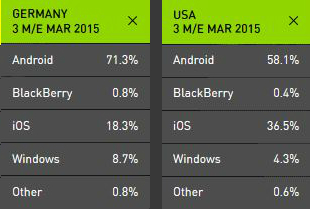
\includegraphics[width=0.5\linewidth]{ios/media/marketshare-cmp-201503.jpg}
		\caption{Marktanteil der mobilen Betriebssysteme
		\cite{MobileOsStat}}
		\label{fig:marcetshare}
	\end{figure}